\documentclass[conference]{IEEEtran}

\usepackage[T1]{fontenc}
\usepackage{graphicx}
\usepackage{booktabs}
\usepackage{amsmath,amssymb}
\usepackage{microtype}
\usepackage{url}
\usepackage[hidelinks]{hyperref}
\usepackage{flushend}
\usepackage{placeins}

% Fig. 1 and Table I are both full-width; at the default dbltopfraction they
% cannot share a page top, so both deferred two pages past their reference.
\renewcommand{\dbltopfraction}{0.92}
\renewcommand{\dblfloatpagefraction}{0.7}
\renewcommand{\textfraction}{0.06}
\setcounter{dbltopnumber}{3}
% four floats x default separation is a lot of vertical space; tighten it
% rather than shrink the figures (their axis labels are already near the
% legibility floor at these widths).
\setlength{\dbltextfloatsep}{10pt plus 2pt minus 2pt}
\setlength{\textfloatsep}{10pt plus 2pt minus 2pt}
\setlength{\dblfloatsep}{8pt plus 2pt minus 2pt}
\setlength{\floatsep}{8pt plus 2pt minus 2pt}
\setlength{\abovecaptionskip}{4pt}
\setlength{\belowcaptionskip}{0pt}

\hypersetup{
    pdftitle={Diagnosing Zero-Shot Forgetting in CLIP Fine-Tuning: Attention Drift Characterizes Adaptation, Representation Drift Predicts Transfer Degradation},
    pdfauthor={Ruize Xia},
    pdfkeywords={CLIP, attention, fine-tuning, LoRA, catastrophic forgetting, vision transformers}
}

\title{Diagnosing Zero-Shot Forgetting in CLIP Fine-Tuning:\\
Attention Drift Characterizes Adaptation,\\
Representation Drift Predicts Transfer Degradation}

\author{\IEEEauthorblockN{Ruize Xia}
\IEEEauthorblockA{\textit{High School Student, Nanjing Foreign Language School}\\
Nanjing, Jiangsu, China\\
xiaruize0911@gmail.com}}

\begin{document}
\maketitle

\begin{abstract}
Contrastive Language--Image Pretraining (CLIP) supports zero-shot classification---prediction from natural-language class descriptions---but fine-tuning can erode this transfer \cite{radford2021learning,kumar2022finetuning}. We test whether such degradation can be anticipated from unlabeled target images. Six label-free signals are evaluated: class-token attention entropy, effective receptive field, Gini concentration, centered kernel alignment (CKA) \cite{kornblith2019similarity}, embedding drift, and relative weight change. The primary controlled experiment compares conventional full fine-tuning (Full FT) with low-rank adaptation (LoRA) \cite{hu2022lora} across two datasets, four matched learning rates, and three random seeds under leakage-free checkpoint selection; a second-backbone extension tests robustness. Optimization scale controls the magnitude but not the direction of attention change. Signed entropy change is the strongest within-group correlate of forgetting (mean absolute rank correlation 0.860), yet its sign varies across backbone--method groups and its cross-configuration correlation is only 0.361. By contrast, CKA and embedding drift maintain consistent relationships with retention and remain informative after one epoch. Attention drift therefore characterizes the intensity and location of adaptation, whereas representation drift more reliably indicates transfer degradation.
\end{abstract}

\begin{IEEEkeywords}
CLIP, attention, fine-tuning, LoRA, catastrophic forgetting, vision transformers
\end{IEEEkeywords}

\section{Introduction}
CLIP acquires broadly transferable visual representations from natural-language supervision \cite{radford2021learning}, yet task-specific fine-tuning can trade that generality for in-domain accuracy \cite{kumar2022finetuning}. This trade-off is usually quantified retrospectively on a benchmark approximating the pretraining distribution. Such evaluation may be computationally costly, unavailable in specialized applications, or impossible when suitable labels do not exist.

We therefore ask whether transfer degradation can be anticipated from internal model changes measured on unlabeled target images. The motivating observation is that attention from CLIP's class (CLS) token to its image-patch tokens often contracts under aggressive fine-tuning and changes less under low-rank adaptation, suggesting attention drift as a potential early-warning statistic. We test this hypothesis against representation- and weight-based alternatives and identify the conditions under which each diagnostic is reliable.

\textbf{Contributions.}
\begin{enumerate}
    \item A leakage-free, auditable dose-response analysis comprising 66 runs with a Vision Transformer Base using $32\!\times\!32$-pixel patches (ViT-B/32) and 18 runs using $16\!\times\!16$-pixel patches (ViT-B/16).
    \item A comparative evaluation of label-free drift signals under three criteria: final rank correlation, prediction from the first epoch, and configuration-selection utility.
    \item Evidence that signed attention-entropy drift is reliable within a fixed dataset--method--backbone group but unstable across groups; it measures adaptation \emph{dose} more reliably than transfer \emph{damage}.
    \item Reference configurations, a frozen-projection ablation, and an exploratory interpolation intervention that characterize the accuracy--retention frontier.
\end{enumerate}

\section{Related Work}
\textbf{Adapting CLIP without breaking it.}
Conventional fine-tuning can distort pretrained features and degrade out-of-distribution performance \cite{kumar2022finetuning}. Existing remedies modify either the parameters or the objective, including interpolation between zero-shot and fine-tuned models \cite{wortsman2022robust}, task arithmetic \cite{ilharco2023editing}, fine-tuning with the pretraining loss \cite{goyal2023finetune}, and low-rank adaptation \cite{hu2022lora}. These methods are generally evaluated by endpoint accuracy on held-out benchmarks; our focus is instead on signals measurable \emph{during} adaptation from unlabeled target data.

\textbf{What the signals come from.}
Vision transformers expose attention distributions over spatial tokens \cite{dosovitskiy2021image}; because attention weights are not causal explanations \cite{jain2019attention,wiegreffe2019attention}, we treat them only as structural measurements. Zhai et al.\ associate attention-entropy collapse with unstable transformer \emph{training} \cite{zhai2023stabilizing}; we test whether the same statistic tracks degradation during \emph{adaptation}. Since concentrated attention can be normal in trained transformers \cite{xiao2024efficient,darcet2024vision}, all attention statistics are expressed relative to the pretrained model. For representation-level comparison, centered kernel alignment (CKA) measures model similarity \cite{kornblith2019similarity}, while the projection norm links update magnitude to out-of-distribution error \cite{yu2022predicting}. We place attention, representation, and weight drift in a common evaluation of lost pretrained capability.

\section{Method}
\subsection{Label-Free Drift Signals}
All signals are computed on a fixed set of unlabeled target-domain images, termed the \emph{probe set}. Consequently, each diagnostic requires only the data already available for fine-tuning.

For block $\ell$, attention head $h$, and a probe image, let $a_{\ell h}$ denote class-token attention over $N_p$ patch tokens ($N_p=49$ for ViT-B/32 and 196 for ViT-B/16), renormalized after removing class-token self-attention. Entropy, measured with natural logarithms (nats), is
\begin{equation}
H(a_{\ell h})=-\sum_{j=1}^{N_p}a_{\ell hj}\log a_{\ell hj},
\end{equation}
and is averaged over images, heads, and the 12 transformer blocks. The effective receptive field at a 95\% attention-mass threshold (ERF@0.95) is the fraction of patches required, in descending attention order, to accumulate 95\% of the mass; the Gini coefficient provides a second measure of concentration. For any quantity $M$, relative drift from the pretrained model is
\begin{equation}
\Delta M = 100\,\frac{M_{\mathrm{adapted}}-M_{\mathrm{pretrained}}}{M_{\mathrm{pretrained}}}.
\end{equation}
We report both block-averaged $\Delta H$ and last-block $\Delta H_{12}$ because averaging can conceal opposite-signed layerwise changes.

We compare three non-attention signals. Relative encoder-weight change, the corresponding LoRA update, and embedding drift are defined as
\begin{align}
D_W &= \frac{\lVert\Delta W\rVert_2}{\lVert W_0\rVert_2},
& \Delta W_{\mathrm{LoRA}} &= \frac{\alpha}{r}BA, \\
D_z &= 1-\cos(z_0,z).
\end{align}
The LoRA form places both methods on a common scale and requires no forward pass. \emph{CKA} is the blockwise mean linear centered kernel alignment \cite{kornblith2019similarity} between pretrained and adapted class-token activations. Target-task training loss and accuracy serve as baselines; only accuracy requires labels.

\subsection{Primary Controlled Experiment}
The primary controlled experiment uses a leakage-free protocol, includes reference configurations, and records every signal at each epoch. It uses the EuroSAT land-use dataset \cite{helber2019eurosat} and the Oxford-IIIT Pets dataset (Pets) \cite{parkhi2012cats}. Validation sets (300 EuroSAT and 370 Pets images) and unlabeled probe sets (200 and 222 images) are drawn from the training split and are mutually disjoint from the training subset. The provided test split is evaluated once per run, using the checkpoint selected by validation accuracy. Training uses fixed class-balanced subsets (1{,}600 and 1{,}480 images), batch size 32, six epochs, the AdamW optimizer (Adam with decoupled weight decay) with weight decay 0.01, 5\% linear warmup followed by cosine decay, and gradient clipping at 1.0. The matched learning-rate grid $\{3\cdot 10^{-6},10^{-5},3\cdot 10^{-5},10^{-4}\}$ spans weak to strongly damaging adaptation under this shorter schedule. Random seeds are $\{7,11,19\}$. Each run record includes its complete per-epoch history, and the released analysis script regenerates all reported tables, statistics, and figures.\footnote{Code and per-run records: \url{https://github.com/xiaruize0911/Attention_Collapse_in_CLIP_Fine-tuning_repo}}

All ViT-B/32 experiments freeze the text encoder. Conventional full fine-tuning (Full FT) updates the visual encoder, visual projection, and a linear classifier. Low-rank adaptation (LoRA) inserts rank-8 trainable updates ($\alpha=16$, dropout 0.05) into each visual query and value projection and also trains the projection and classifier. References include a \emph{linear probe} (encoder and projection frozen), \emph{last-block} fine-tuning (final block and output layer normalization), and \emph{LoRA with a frozen visual projection}. A backbone-robustness extension repeats the EuroSAT grid at three learning rates on ViT-B/16 (18 runs). The intervention interpolates encoder and projection parameters while retaining the adapted classifier:
\begin{equation}
\theta(\alpha)=(1-\alpha)\theta_0+\alpha\theta_1.
\end{equation}

\subsection{Transfer-Retention Outcome and Evaluation}
Zero-shot transfer is evaluated through the active, adapter-aware image encoder. The selected model produces image embeddings that are matched against text embeddings of ``a photo of a \{class\}.'' This implementation detail is essential: evaluating a LoRA checkpoint through an unmodified CLIP instance returns the pretrained pathway rather than the adapted model. We report CIFAR-100 \cite{krizhevsky2009learning} (all 10{,}000 test images) and CIFAR-10 (2{,}000 balanced images) as \emph{retention}, defined as the percentage of pretrained zero-shot accuracy preserved; pretrained accuracies are 61.33\% and 87.40\%, respectively. The two rank runs almost identically ($\rho=0.971$, $n=48$), so the body reports CIFAR-100 alone; retention above 100\% means accuracy above the pretrained level.

Each signal is evaluated by (i) Spearman rank correlation with final CIFAR-100 retention, (ii) the corresponding correlation using only its first-epoch value, and (iii) selection utility. For the third criterion, a signal selects among runs within two percentage points of the best validation accuracy, and the retained zero-shot performance is compared with the best achievable value in that candidate set (the oracle value).

\begin{figure*}[!t]
    \centering
    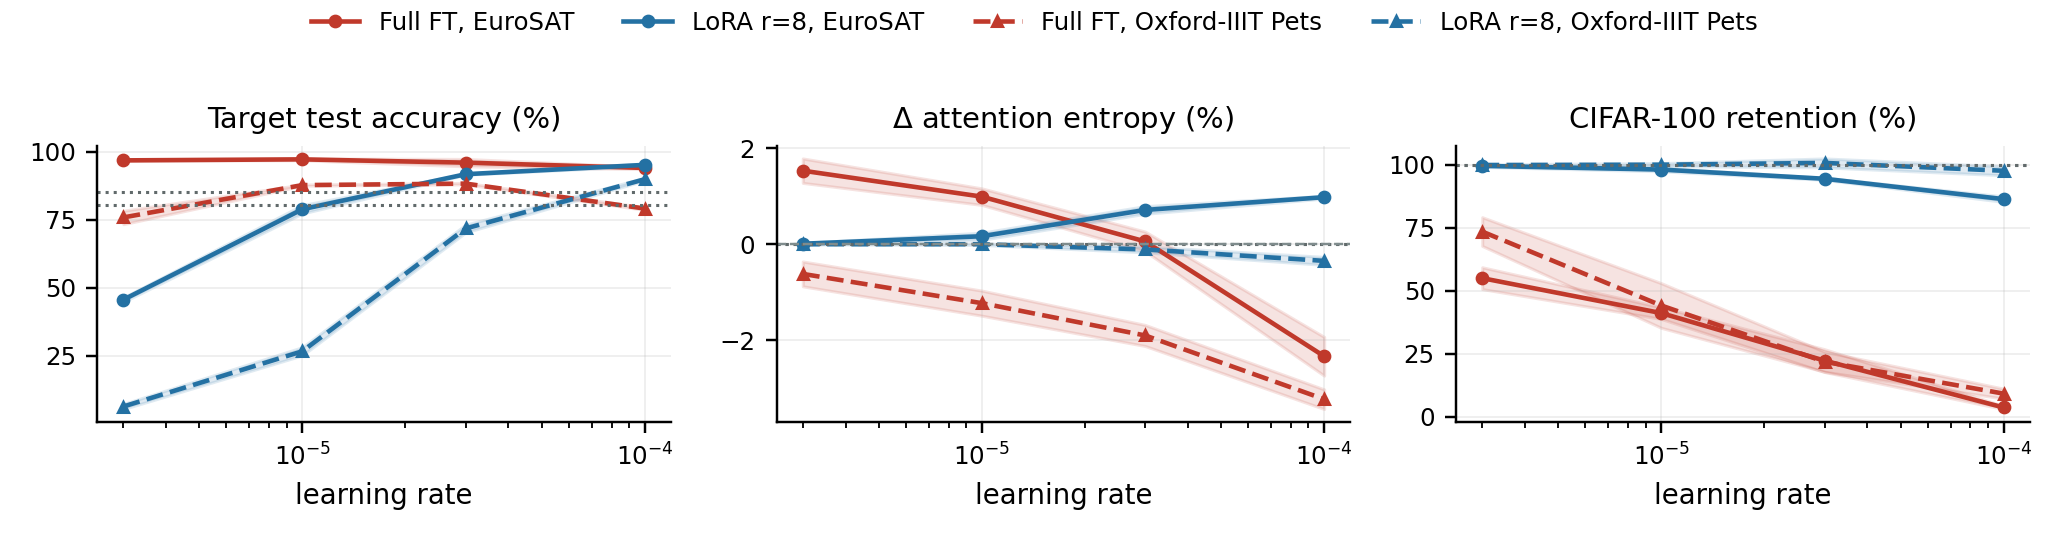
\includegraphics[width=0.78\textwidth]{figures/study2_dose_response.png}
    \caption{Dose-response in the primary controlled experiment. Curves show means over three seeds, shaded regions one standard deviation, and dotted lines the linear-probe reference. On EuroSAT, Full FT crosses from attention broadening to contraction (center), whereas LoRA entropy increases with learning rate; retention nevertheless declines for both methods.}
    \label{fig:dose}
\end{figure*}

\begin{table*}[!t]
\caption{Primary matched-learning-rate grid: mean $\pm$ across-seed standard deviation over $n$ seeds. $\Delta H$ is the block-averaged entropy change from pretrained CLIP, $\Delta H_{12}$ the last-block change; retention is the surviving percentage of pretrained zero-shot accuracy (61.33\% on CIFAR-100; CIFAR-10 ranks runs almost identically, $\rho=0.971$). Test accuracy is read once, at the validation-selected epoch.}
\label{tab:grid}
\centering
\scriptsize
\setlength{\tabcolsep}{4pt}
\renewcommand{\arraystretch}{0.85}
\begin{tabular}{llrrrrrr}
\toprule
Dataset & Method & Learning rate & $n$ & Test accuracy (\%) & $\Delta H$ (\%) & $\Delta H_{12}$ (\%) & CIFAR-100 retention (\%) \\
\midrule
EuroSAT & Full FT & $3\cdot 10^{-6}$ & 3 & 96.81\,$\pm$\,0.07 & 1.53\,$\pm$\,0.25 & 3.39\,$\pm$\,0.38 & 55.03\,$\pm$\,4.33 \\
EuroSAT & Full FT & $10^{-5}$ & 3 & 97.19\,$\pm$\,0.33 & 0.99\,$\pm$\,0.17 & 1.24\,$\pm$\,0.36 & 41.15\,$\pm$\,2.31 \\
EuroSAT & Full FT & $3\cdot 10^{-5}$ & 3 & 95.98\,$\pm$\,1.36 & 0.06\,$\pm$\,0.21 & -2.39\,$\pm$\,0.48 & 22.27\,$\pm$\,4.52 \\
EuroSAT & Full FT & $10^{-4}$ & 3 & 94.02\,$\pm$\,0.43 & -2.34\,$\pm$\,0.40 & -7.75\,$\pm$\,2.87 & 3.65\,$\pm$\,0.62 \\
EuroSAT & LoRA r=8 & $3\cdot 10^{-6}$ & 3 & 45.54\,$\pm$\,0.80 & 0.01\,$\pm$\,0.02 & 0.00\,$\pm$\,0.08 & 99.65\,$\pm$\,0.42 \\
EuroSAT & LoRA r=8 & $10^{-5}$ & 3 & 78.83\,$\pm$\,1.54 & 0.16\,$\pm$\,0.07 & 0.37\,$\pm$\,0.33 & 98.18\,$\pm$\,0.69 \\
EuroSAT & LoRA r=8 & $3\cdot 10^{-5}$ & 3 & 91.73\,$\pm$\,0.19 & 0.71\,$\pm$\,0.08 & 2.04\,$\pm$\,0.38 & 94.52\,$\pm$\,0.41 \\
EuroSAT & LoRA r=8 & $10^{-4}$ & 3 & 95.16\,$\pm$\,0.44 & 0.98\,$\pm$\,0.03 & 1.71\,$\pm$\,0.27 & 86.44\,$\pm$\,1.09 \\
Oxford-IIIT Pets & Full FT & $3\cdot 10^{-6}$ & 3 & 75.82\,$\pm$\,2.47 & -0.62\,$\pm$\,0.26 & -4.95\,$\pm$\,0.38 & 73.54\,$\pm$\,5.71 \\
Oxford-IIIT Pets & Full FT & $10^{-5}$ & 3 & 87.72\,$\pm$\,0.20 & -1.23\,$\pm$\,0.26 & -6.97\,$\pm$\,0.48 & 44.17\,$\pm$\,8.87 \\
Oxford-IIIT Pets & Full FT & $3\cdot 10^{-5}$ & 3 & 88.26\,$\pm$\,0.26 & -1.90\,$\pm$\,0.22 & -10.30\,$\pm$\,0.62 & 21.83\,$\pm$\,3.98 \\
Oxford-IIIT Pets & Full FT & $10^{-4}$ & 3 & 79.10\,$\pm$\,0.49 & -3.23\,$\pm$\,0.20 & -18.51\,$\pm$\,1.29 & 9.16\,$\pm$\,1.96 \\
Oxford-IIIT Pets & LoRA r=8 & $3\cdot 10^{-6}$ & 3 & 6.23\,$\pm$\,0.93 & -0.00\,$\pm$\,0.00 & -0.01\,$\pm$\,0.02 & 99.98\,$\pm$\,0.27 \\
Oxford-IIIT Pets & LoRA r=8 & $10^{-5}$ & 3 & 26.56\,$\pm$\,1.50 & -0.00\,$\pm$\,0.01 & -0.08\,$\pm$\,0.10 & 100.11\,$\pm$\,0.62 \\
Oxford-IIIT Pets & LoRA r=8 & $3\cdot 10^{-5}$ & 3 & 71.75\,$\pm$\,1.42 & -0.11\,$\pm$\,0.06 & -2.03\,$\pm$\,0.47 & 100.82\,$\pm$\,1.77 \\
Oxford-IIIT Pets & LoRA r=8 & $10^{-4}$ & 3 & 89.88\,$\pm$\,0.47 & -0.35\,$\pm$\,0.08 & -5.94\,$\pm$\,0.44 & 97.70\,$\pm$\,1.78 \\
\bottomrule
\end{tabular}
\end{table*}

\section{Results}
\subsection{Optimization Scale Sets the Magnitude of Drift}
Fig.~\ref{fig:dose} and Table~\ref{tab:grid} show that learning rate systematically affects both attention structure and retention, although the direction of attention change depends on the adaptation method. On EuroSAT, Full FT \emph{broadens} attention at the smallest matched rate (1.53\,$\pm$\,0.25\%), is approximately neutral at $3\cdot 10^{-5}$ (+0.06\%), and contracts at $10^{-4}$ (-2.34\%); the rate-dependent trend is monotonic (Spearman $\rho=-0.972$; $p=1.4\cdot 10^{-7}$). LoRA exhibits the opposite trend, with entropy increasing from +0.01\% to +0.98\% ($\rho=0.972$). On Pets, both methods are contractive: Full FT changes from -0.62\% to -3.23\%, and LoRA from -0.00\% to -0.35\%.

CIFAR-100 retention declines with learning rate in three of the four groups (Spearman $\rho=-0.972$ in each): from 55.0\% to 3.7\% for EuroSAT Full FT and from 99.6\% to 86.4\% for LoRA. The exception is LoRA on Pets, for which retention remains near the pretrained level throughout the grid (100.0\% to 97.7\%; $\rho=-0.324$; $p=0.30$). Thus, entropy change is not a configuration-independent measure of damage: on EuroSAT, both methods reach $\Delta H\approx+1\%$ despite markedly different retention.

Paired over identical (learning rate, seed) cells, LoRA keeps 64.2 percentage points more of pretrained CIFAR-100 accuracy than Full FT on EuroSAT ($p=2.0\cdot 10^{-7}$ after Holm adjustment for multiple comparisons; paired standardized effect size $|d_z|=4.14$) and 62.5 points more on Pets ($p=2.9\cdot 10^{-5}$). It also stays closer to the pretrained representation (mean CKA higher by 0.164, $p=3.4\cdot 10^{-12}$). The attention statistic is the weakest discriminator of the two methods and the only one whose verdict depends on the dataset: on EuroSAT the paired difference in $\Delta H$ is 0.41 points at $p=0.49$, while on Pets it is 1.63 points at $p=3.2\cdot 10^{-4}$.

The comparison remains substantial at each method's validation-selected operating point. On EuroSAT, Full FT selects $10^{-5}$ and obtains 97.19\% target accuracy with 41.2\% retention; LoRA selects $10^{-4}$ and obtains 95.16\% accuracy with 86.4\% retention. On Pets, LoRA is superior on both axes: 89.88\% versus 88.26\% target accuracy and 97.7\% versus 21.8\% retention.

\subsection{Predictive Validity of Attention Drift}
Fig.~\ref{fig:predictors} compares signals by their ability to rank runs according to final CIFAR-100 retention. A non-label-free reference---retention on a labeled 1{,}000-image subset \emph{of the evaluation set itself}, read after one epoch---reaches $\rho=0.967$; sharing 10\% of its images with the predicted quantity, it is an optimistic ceiling rather than a fair competitor. Among label-free signals, CKA (0.960) and embedding drift (-0.919) lead; a middle tier spanning $|\rho|$ from 0.877 to 0.796 holds last-block CKA, $|\Delta$Gini$|$, relative weight change (-0.837), $|\Delta H|$ (-0.836), $|\Delta$ERF@0.95$|$ and the training loss (0.824), which fine-tuning computes anyway. Target-task accuracy correlates at -0.606, while signed entropy change---the statistic motivating this study---reaches only 0.361 across configurations.
\begin{figure}[!t]
    \centering
    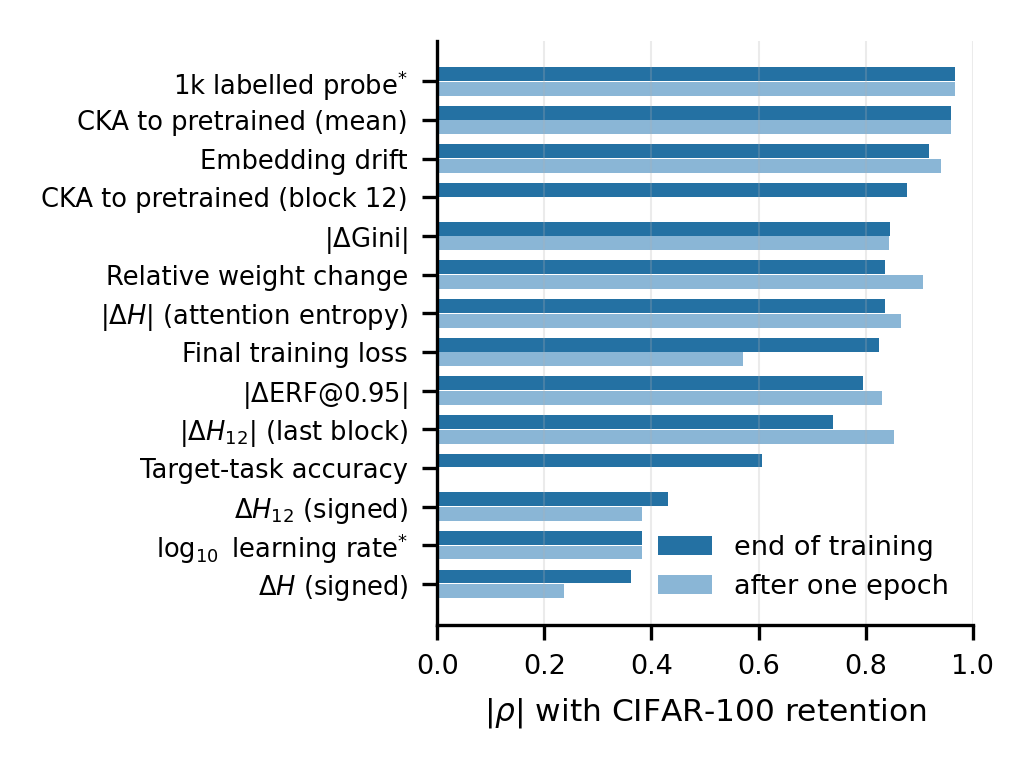
\includegraphics[width=0.9\columnwidth]{figures/study2_predictor_bars.png}
    \caption{Absolute Spearman correlation with final CIFAR-100 retention across core runs, measured at the end of training (dark) and after one epoch (light). Missing bars indicate signals without an epoch-1 counterpart. $^{*}$The labeled probe is not label-free; learning rate is a hyperparameter rather than a measured signal. Across configurations, attention statistics are intermediate predictors and signed entropy drift is weak.}
    \label{fig:predictors}
\end{figure}


To avoid treating seeds within a configuration as independent evidence, uncertainty is estimated by resampling the 16 cell means. Of the 10 paired comparisons---uncorrected, so only the largest should be read as firm---CKA's advantage excludes zero relative to signed $\Delta H$ (+0.601; 95\% confidence interval (CI) [0.149, 0.948]) and $|\Delta H_{12}|$ (+0.226 [0.030, 0.573]), but not relative to embedding drift, $|\Delta H|$, final training loss, or weight change (for the latter: +0.144 [-0.018, 0.424]); it also excludes zero against target accuracy and learning rate, neither label-free. At this sample size, the representation probes lead on point estimates, but their advantage over the strongest lower-cost alternatives is not statistically resolved.

Within a fixed dataset and method, where learning rate is the principal varying factor, the ordering changes. Signed entropy drift becomes the strongest signal (mean $|\rho|=0.860$ over four primary groups), ahead of relative weight change (0.823), log learning rate (0.810), then signed $\Delta H_{12}$, CKA (0.787) and embedding drift between 0.788 and 0.752, with $|\Delta H|$ last (0.656). That ranking is oracle-oriented, taking each correlation's absolute value after its sign is known. Fixing one direction in advance, as a deployable rule must, leaves signed entropy drift at +0.385 while CKA and weight change lose nothing (+0.787, -0.823). Attention drift therefore measures adaptation \emph{dose} effectively when its direction is fixed, but is unreliable as a cross-configuration \emph{damage} measure. These correlations are effect sizes rather than significance tests because each group contains only three or four dose levels. Fig.~\ref{fig:synthesis}(a) summarizes the backbone extension: signed entropy drift changes from strongly positive to negative or null across the four backbone--method groups, whereas CKA and embedding drift keep one direction and relative weight change keeps the other.

This limitation affects selection. Within two points of the best EuroSAT validation accuracy, retention spans 17.1--58.1\% versus 41.2\% under random selection. Embedding drift, weight change, CKA, and $|\Delta H|$ select 56.9\%, 56.9\%, 50.1\%, and 24.0\%, respectively; on Pets, $|\Delta H|$ selects the best configuration. Every EuroSAT candidate here is Full FT; LoRA enters only at wider margins, where the oracle rises to 87.6\%. Across eight dataset--band cases, only CKA and embedding drift remain consistently near the oracle; $|\Delta H|$ is below random in every EuroSAT band, while weight change reaches at most 54.4\% on Pets where 99.7\% is achievable.

The representation-level signals are also informative early in training. After one of six epochs, CKA correlates with final retention at $\rho=0.959$ and relative weight change at $-0.906$. At the configuration level, embedding drift and CKA separate low- and high-retention configurations with an outcome-oriented area under the receiver operating characteristic curve (AUC) of 1.00; relative weight change reaches 0.98, and signed entropy drift reaches 0.68. Because the favorable direction is selected using the outcome, these AUCs are descriptive upper bounds rather than deployment estimates.

\subsection{Attention Drift as a Structural Descriptor}
Attention drift remains informative about \emph{where} adaptation occurs. Under Full FT at $10^{-4}$, $\Delta H_{12}$ reaches -7.7\% on EuroSAT and -18.5\% on Pets, compared with block-averaged changes of -2.3\% and -3.2\%; the first four blocks remain within 1.8\% of pretrained. Layer-resolved entropy drift is therefore a useful structural descriptor and method fingerprint, even when its scalar average is not a reliable damage predictor.

\subsection{The Trade-off Is a Frontier}
Fig.~\ref{fig:synthesis}(b) shows the EuroSAT accuracy--retention frontier. The linear probe anchors the preservation end at 85.1/100.0 accuracy/retention. Six configurations are non-dominated, including Full FT at $10^{-5}$ (97.2/41.2), LoRA at $10^{-4}$ (95.2/86.4), and last-block tuning at $10^{-5}$ (88.6/97.1). The frontier makes clear that neither target accuracy nor structural preservation alone determines a preferred configuration.

Update location also matters. Last-block tuning at $10^{-4}$ changes encoder weights more than Full FT at $3\cdot 10^{-5}$ (0.0109 versus 0.0083) yet retains 83.8\% rather than 22.3\%. Freezing LoRA's visual projection at $10^{-4}$ similarly lowers retention from 86.4\% to 76.6\% and target accuracy from 95.2\% to 92.7\%. Layer location and projection capacity therefore complement scalar drift magnitude.

\begin{figure*}[!t]
    \centering
    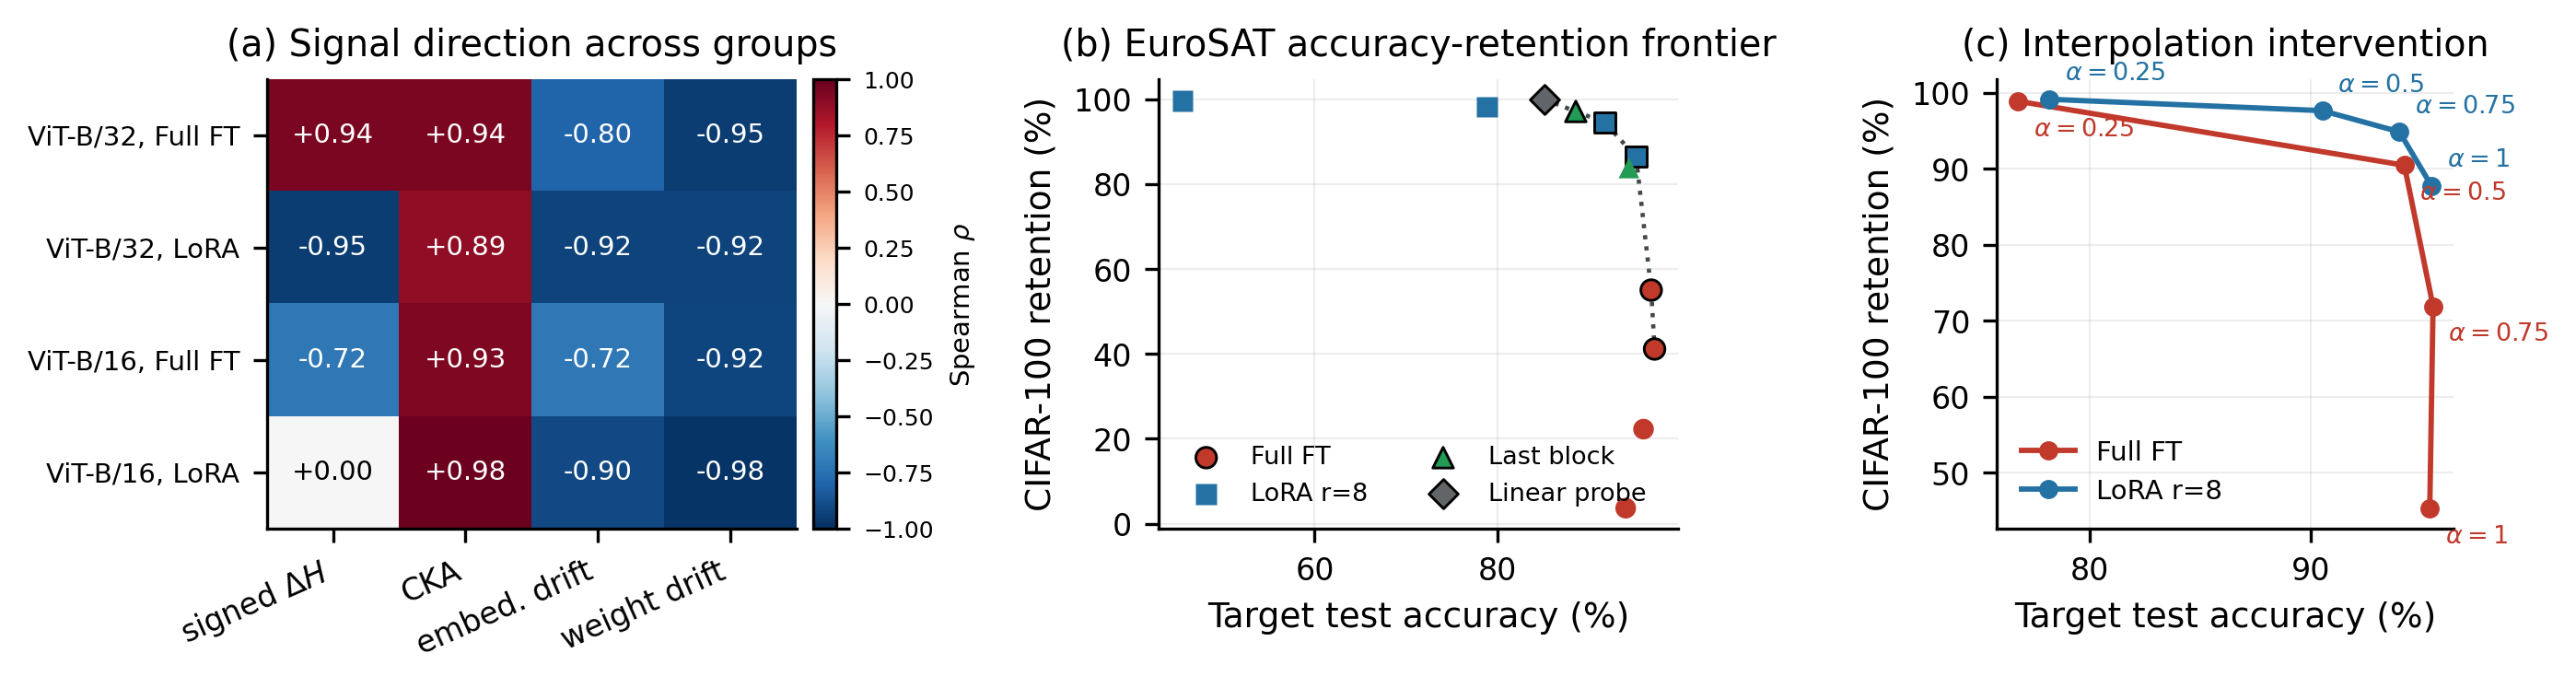
\includegraphics[width=0.98\textwidth]{figures/study2_visual_synthesis.png}
    \caption{Visual synthesis of the principal cross-configuration results. (a) Run-level Spearman correlation with CIFAR-100 retention on EuroSAT: signed attention-entropy drift changes sign across backbone--method groups, while CKA and relative weight change retain consistent directions. (b) EuroSAT cell means in target-accuracy--retention space; black outlines and the dotted line mark non-dominated configurations. (c) Single-seed interpolation trajectories for the validation-selected Full FT and LoRA configurations; $\alpha=0$ is omitted as degenerate.}
    \label{fig:synthesis}
\end{figure*}

\section{Discussion and Limitations}
Three findings remain robust under the leakage-free protocol. First, optimization scale orders structural drift and zero-shot forgetting. Second, LoRA changes the encoder less and preserves substantially more zero-shot performance than Full FT at matched learning rates. Third, contrary to the motivating hypothesis, scalar attention drift is primarily descriptive rather than predictively reliable across configurations.

The limitation of entropy drift is specific: it tracks adaptation dose when its sign is fixed, but that sign depends on the dataset, method, and backbone rather than on damage itself. A cross-configuration selection rule therefore inherits this instability. Representation alignment offers a more reliable practical diagnostic: a few hundred unlabeled target images are sufficient to compare pretrained and adapted encoders, and the signal is informative after one epoch. Relative weight change is less expensive because it requires no images and has a stable sign, but its selection utility is inconsistent; within a five-point band on Pets it selects 54.4\% retention when 99.7\% is available.

The interpolation trajectories in Fig.~\ref{fig:synthesis}(c), following robust fine-tuning \cite{wortsman2022robust}, provide preliminary evidence that this frontier is controllable. For Full FT, $\alpha=0.5$ raises retention from 45.3\% to 90.5\% with only a small accuracy change; for LoRA, $\alpha=0.75$ raises retention from 87.8\% to 94.9\%. The $\alpha=0$ endpoint is omitted as degenerate: the adapted classifier on a pretrained encoder scores near chance. Because each trajectory uses one seed, and the sweep retrains rather than reloading its checkpoint---so $\alpha=1$ replicates its grid cell rather than reproducing it---the intervention is illustrative.

\textbf{Limitations.} The main analysis is correlational, and the interpolation experiment uses one seed and two configurations; causal claims therefore require a replicated intervention. The primary grid covers one backbone, two target datasets, and two transfer benchmarks; the three-seed ViT-B/16 extension is limited to EuroSAT. The grid uses class-balanced subsets and six epochs to stay computationally feasible, so absolute drift magnitudes should be compared only within the same experimental setting. Attention entropy quantifies distributional concentration rather than semantic correctness, and retention uses a single prompt template. Finally, CKA and embedding drift are more proximal to zero-shot predictions than attention entropy; the relevant empirical result is their stability across configurations and at the first epoch.

\section{Conclusion}
This study evaluated attention drift as an early-warning signal for zero-shot forgetting during CLIP fine-tuning. In the leakage-free matched-rate grid, optimization scale is the primary control on both structural change and retention, while LoRA is consistently less damaging than Full FT. Within a fixed dataset--method--backbone group, signed entropy drift correlates strongly with eventual forgetting (mean $|\rho|=0.860$), but its sign changes across configurations; configuration selection based on it can therefore underperform random choice. Layerwise CKA and embedding drift provide the most consistent cross-configuration diagnostics from unlabeled target images and remain informative after one epoch, although their point-estimate advantage over lower-cost alternatives is not statistically resolved across 16 configurations. Attention drift retains a distinct role as a layer-resolved descriptor of where adaptation occurs, rather than as a universal predictor of transfer degradation.

\FloatBarrier
\bibliographystyle{IEEEtran}
\bibliography{references}

\end{document}
